\begin{center}
    \LARGE Supporting Information
\end{center}
An example of the supporting figure environment:\\
\begin{sfig}[H]
    \centering
    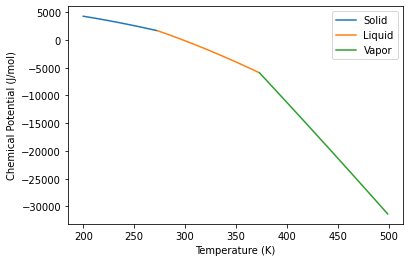
\includegraphics[width=0.5\textwidth,keepaspectratio]{figures/equilibriumplot.png}
    \caption{
    An example of the sfig environment.
    }
    \label{sfig:example}
\end{sfig}
We can also use the subcaption environment here:\\
\begin{sfig}
    \begin{subfigure}{0.45\textwidth}
        \centering
        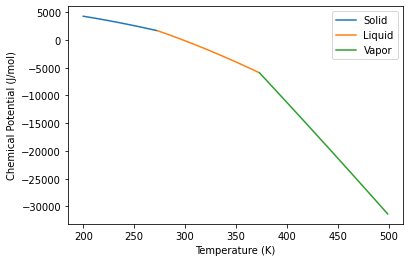
\includegraphics[width=\textwidth,keepaspectratio]{figures/equilibriumplot.png}
        \caption{}
        \label{sfig:sub-example1}
    \end{subfigure}
    \begin{subfigure}{0.45\textwidth}
        \centering
        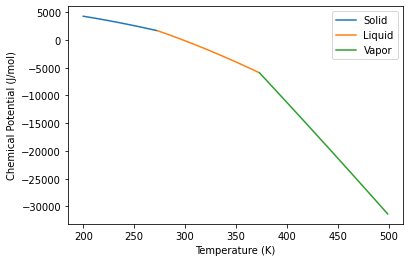
\includegraphics[width=\textwidth,keepaspectratio]{figures/equilibriumplot.png}
        \caption{}
        \label{sfig:sub-example2}
    \end{subfigure}
    \caption{
    An example of subfigures within the sfig environment.
    We can reference each individual figure with subref or ref as we would normally.
    (\subref{sfig:sub-example1}) for example.
    }
    \label{sfig:example-sub-main}
\end{sfig}